%
%  Wakefield Acceleration
% ========================
%

\chapter{The AWAKE Experiment}
\label{Ch:WFA}

AWAKE is the first proton driven wakefield accelerator experiment in the world.
It is a proof-of-concept experiment aiming to inform a design for future high energy accelerators~\cite{gschwendtner:2016} and to prove the feasibility of such an accelerator.
The proton drive beam for the experiment is delivered by the Super Proton Synchrotron (SPS) at CERN at an energy of $400\unit{GeV}$, and joined by an electron witness beam in a $10\unit{m}$ plasma stage.

AWAKE is physically located at the former site of the CERN Neutrinos to Gran Sasso experiment (CNGS) \cite{gschwendtner:2010} in a tunnel below the Swiss-French border, and is connected to the SPS at SPS Point 4.
The connection of the AWAKE experiment to the rest of the CERN accelerator complex is illustrated in Fig.~\ref{Fig:WFA:AccComp}.

\begin{figure}[hbt]
    \centering
    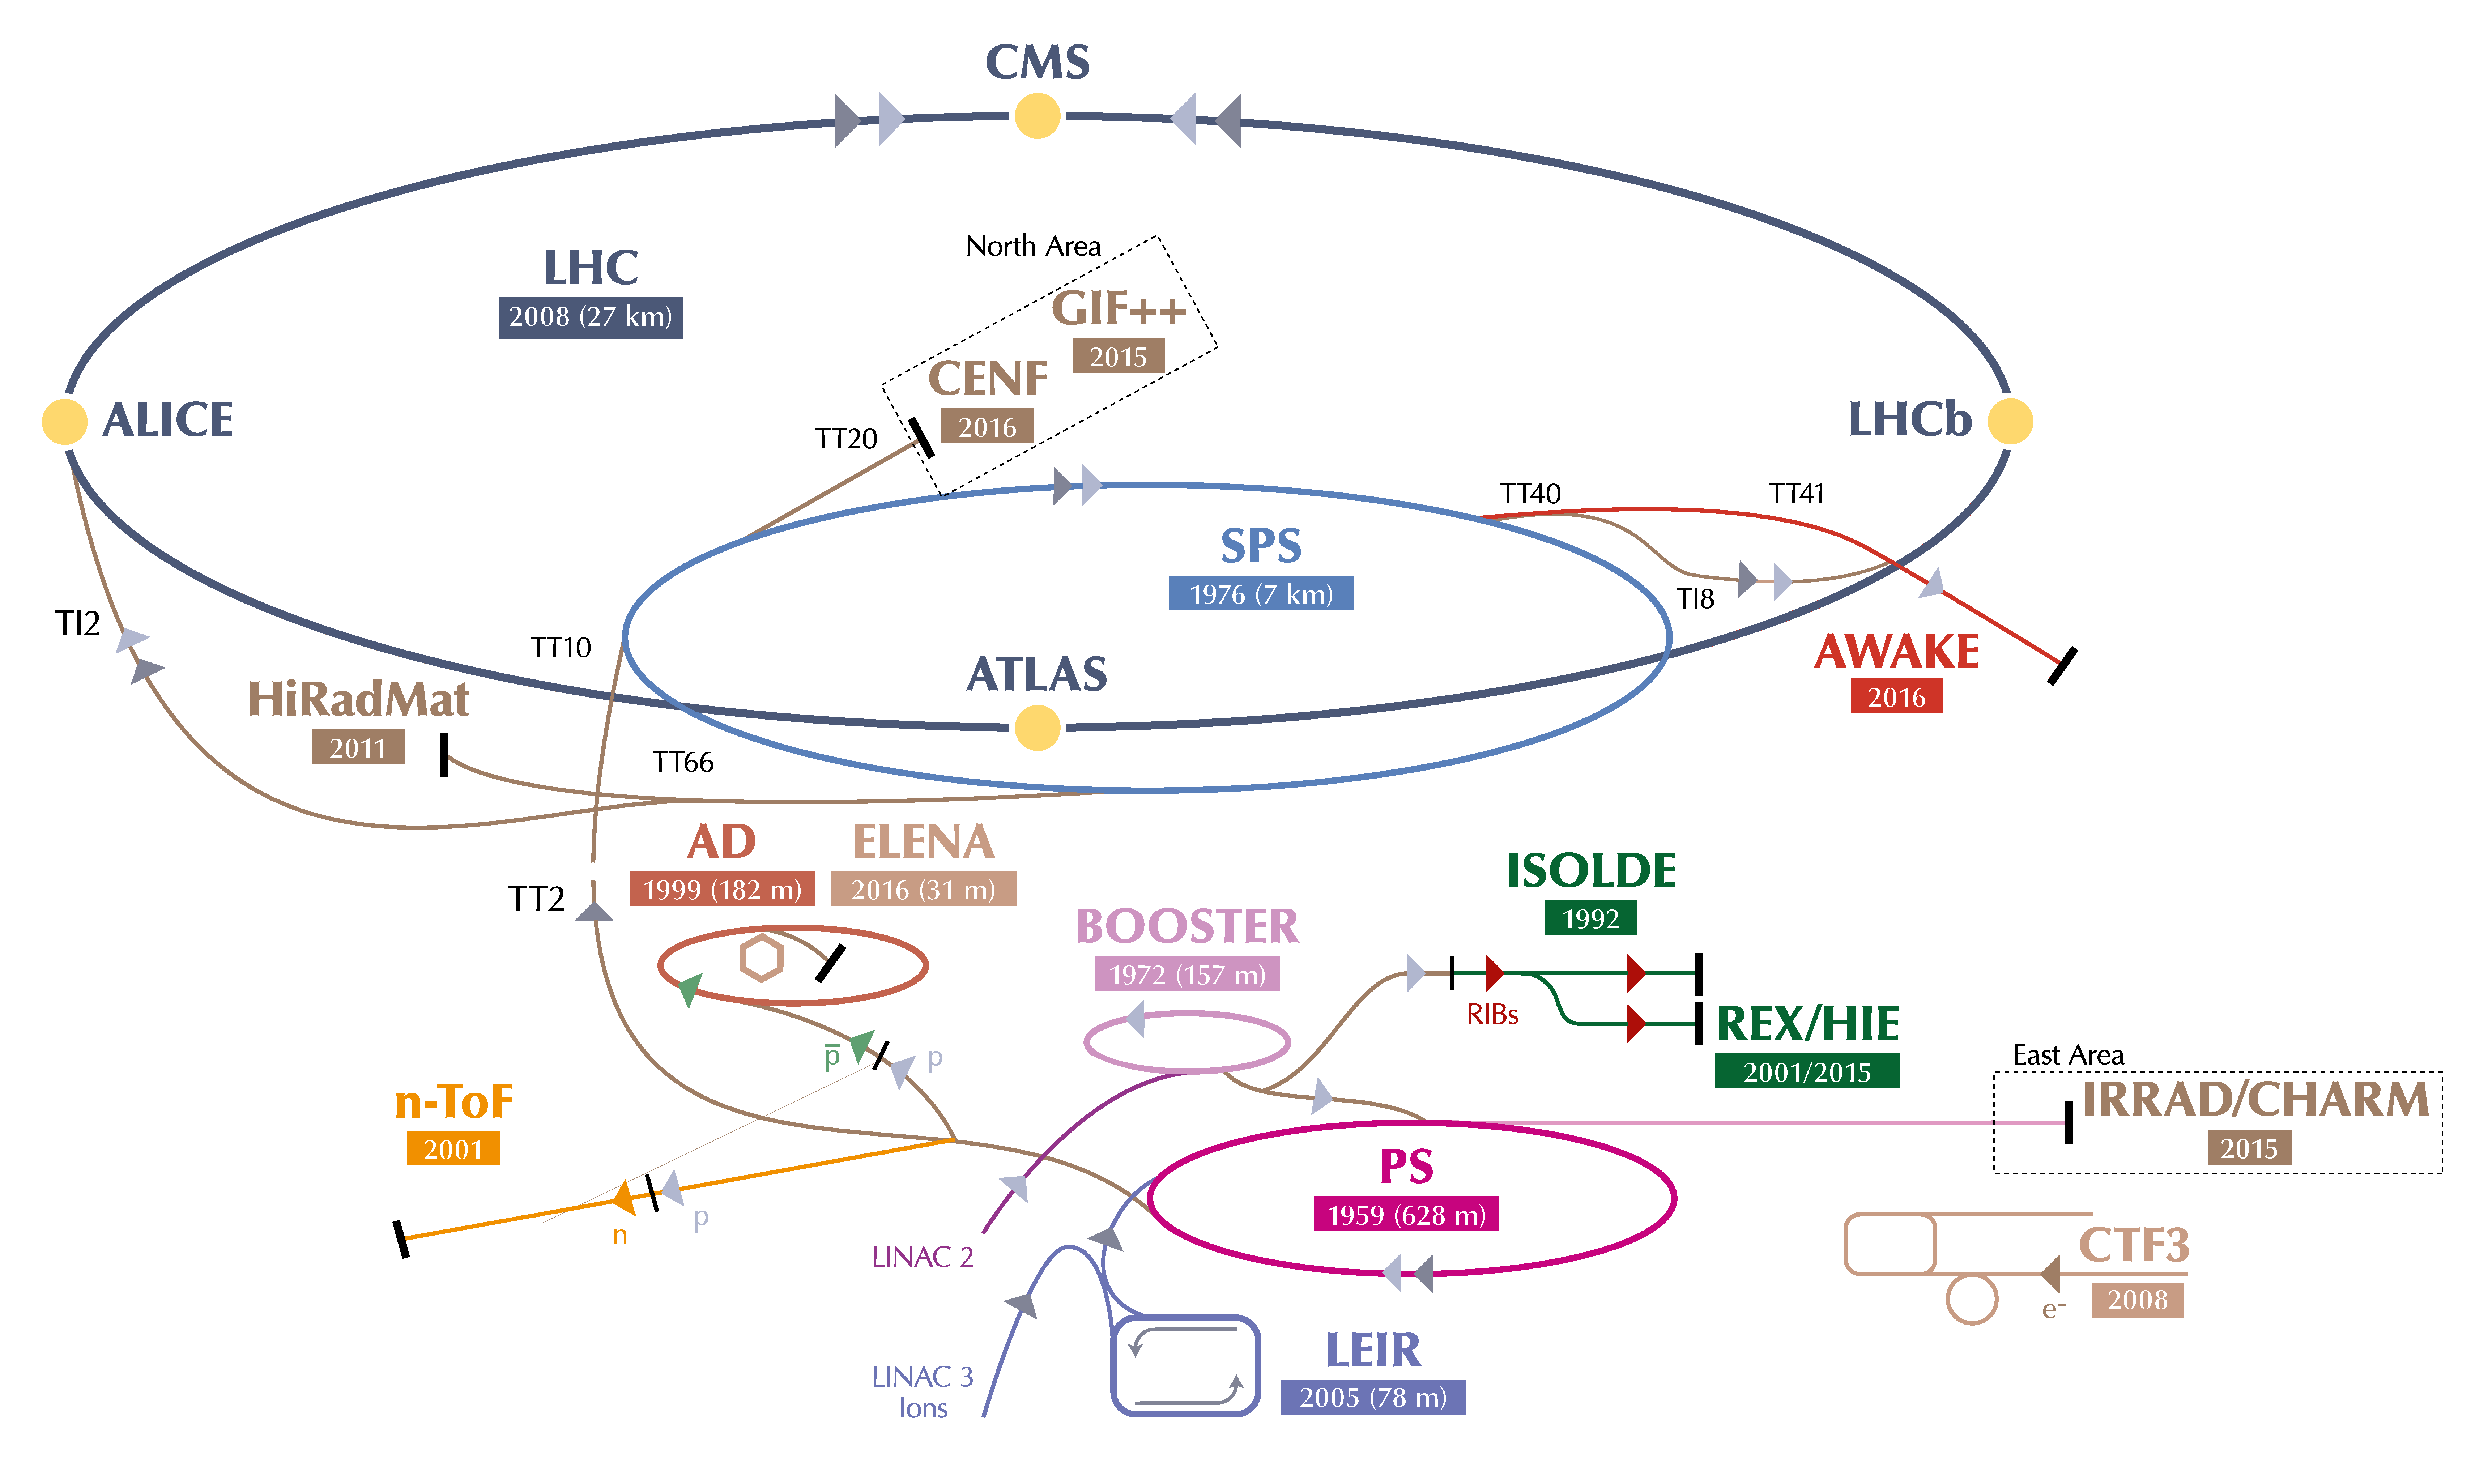
\includegraphics[width=0.99\linewidth,trim={20mm 0mm 20mm 0mm},clip]{figures/AcceleratorComplex}
    \caption{\label{Fig:WFA:AccComp}
        An overview of the CERN Accelerator Complex \cite{add:mobs:2016}.
    }
\end{figure}

% Intro paper \cite{caldwell:2009}
% Launch paper \cite{awake_collaboration:2014}
% Evolution paper \cite{caldwell:2016}
% Technical specifications including simulation parameters \cite{gschwendtner:2016}
% Collaboration paper by Patric \cite{muggli:2017a}

% ================================================================================================================================ %
\section{Evolution of the Concept}
\label{WFA:History}

While AWAKE is the first proton driven wakefield experiment, a number of experiments with electron drive beams have confirmed the models produced by theory and simulations.
The first experimental results of plasma wakefield acceleration were conducted at the Advanced Accelerator Test Facility at Argonne National Laboratory (ANL) outside Chicago, USA, and published in 1988~\cite{rosenzweig:1988}.
The experiment split an electron beam of a few $\unit{nC}$ into a drive and a witness beam, and demonstrated that the drive beam generates accelerating wakefields as well as strong transverse fields. The accelerating gradient they produced was modest, only a few $\unit{MeV}$.

More recently, $\unit{GeV}$ level acceleration gradients have been achieved with an electron bunch at SLAC, where parts of a $42\unit{GeV}$ electron bunch saw energy doubling in an $85\unit{cm}$ plasma cell.
The results were published in Nature in 2007~\cite{blumenfeld:2007}. The plasma stage produced a continuous spread in energy up to about $85\unit{GeV}$.
However, only a small fraction of the charge was accelerated to these energies.
An experiment at SLAC later produced a discrete, accelerated bunch with a core of $74\unit{pC}$ in an accelerating gradient of $4.4\unit{GeV/m}$~\cite{litos:2014}.

%Self modulation at FACET \cite{adli:2016}
%Review by Patric \cite{muggli:2009}

% ================================================================================================================================ %
\section{AWAKE: A Design Overview}
\label{WFA:Design}

AWAKE is, as of the writing of this thesis, operational and in Run~1.
The proton beam line arriving from the SPS joins with the laser beam and the electron beam line, and connects to a $10\unit{m}$ plasma stage at the end of the tunnel.
In addition, an electron source has been installed, and a new side tunnel had to be dug to fit the electron beam line connecting the source to the main assembly.
Figure \ref{Fig:WFA:AWAKE} gives and overview of the experimental layout in the tunnel.
The old CNGS target is still present behind a shielding wall, as it is highly radioactive.
This, unfortunately, has created some constraints for fitting the downstream beam line and diagnostics, and may pose additional challenges for Run~2 if longer or multiple plasma stages are needed.

\begin{figure}[hbt]
    \centering
    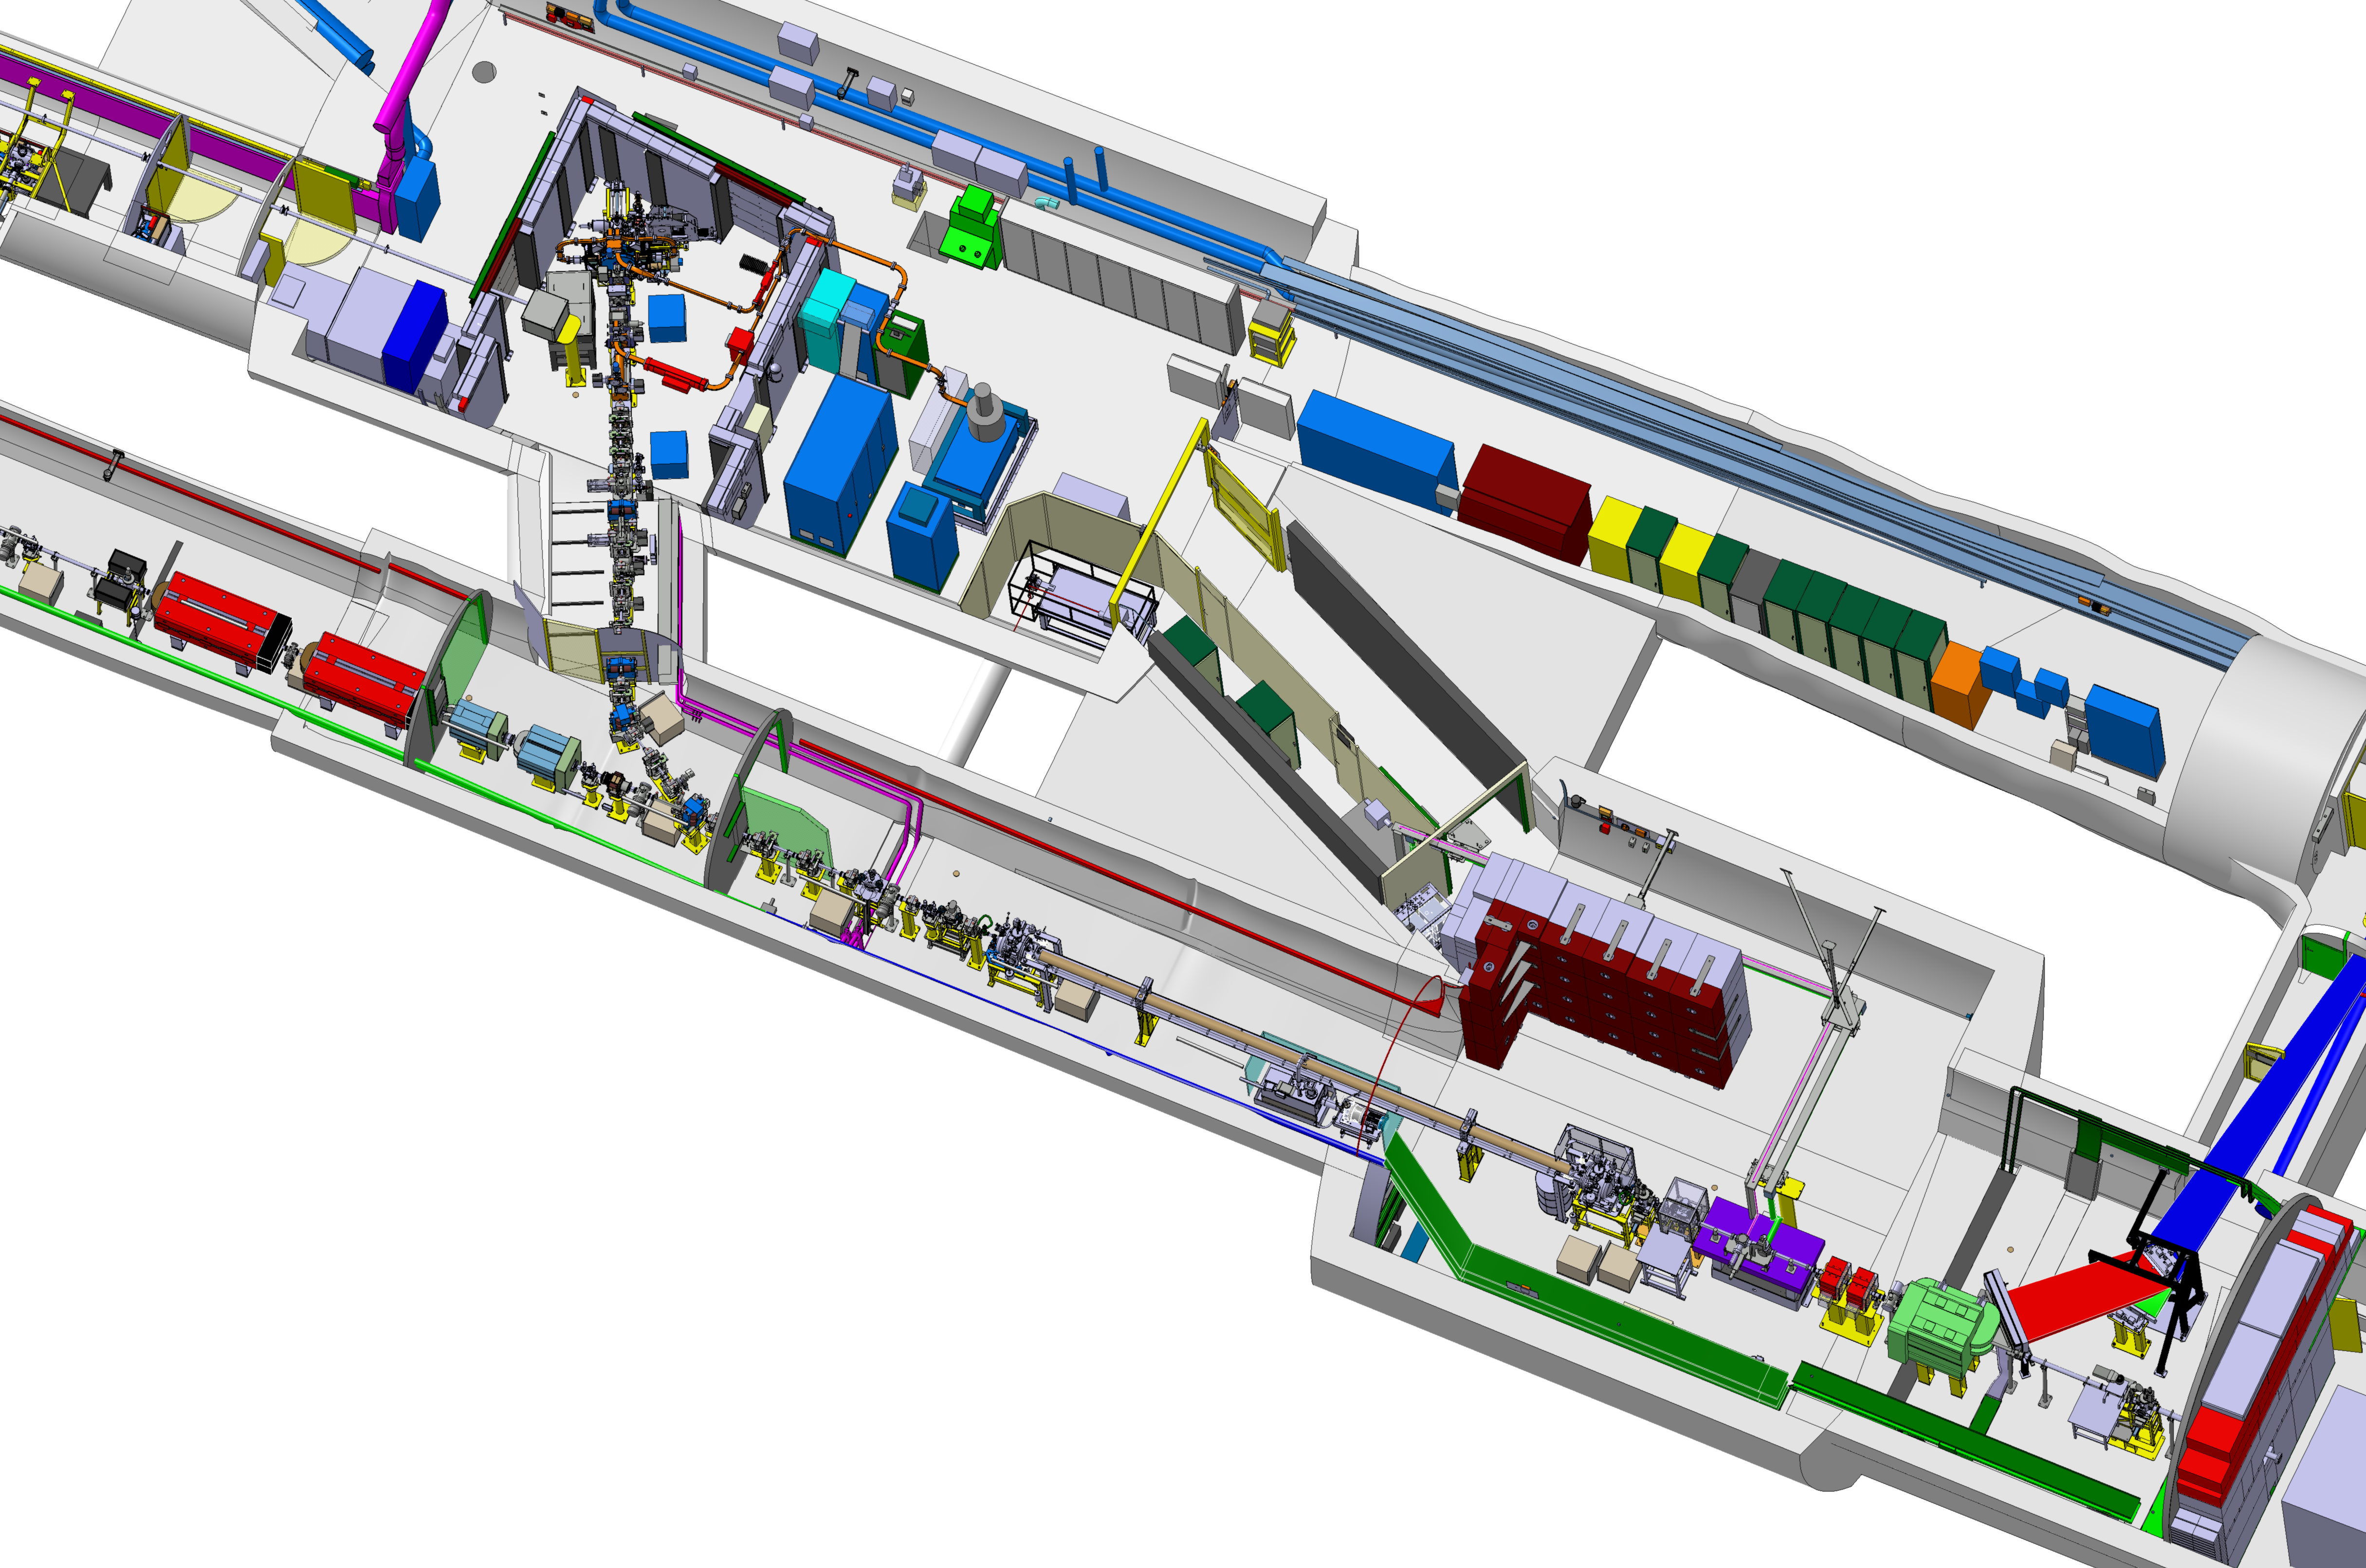
\includegraphics[width=0.99\linewidth,trim={0mm 0mm 0mm 0mm},clip]{figures/AwakeExperiment}
    \caption{\label{Fig:WFA:AWAKE}
        Drawing of the AWAKE experimental area with the key components labelled.
    }
\end{figure}

% ================================================================================================================================ %
\subsection{Plasma Source}
\label{WFA:Design:Plasma}

The requirements for the plasma source for AWAKE Run~1 were a $10\unit{m}$ long cell capable of a plasma electron density ranging from $1-10\nexp{14}\unit{cm}^{-3}$.
The density variation should be within $0.2\%$, and the radius of the plasma channel should be $\geq 1\unit{mm}$.
The plasma should also consist of heavy ions to mitigate ion motion~\cite{caldwell:2015}.

\begin{figure}[hbt]
    \centering
    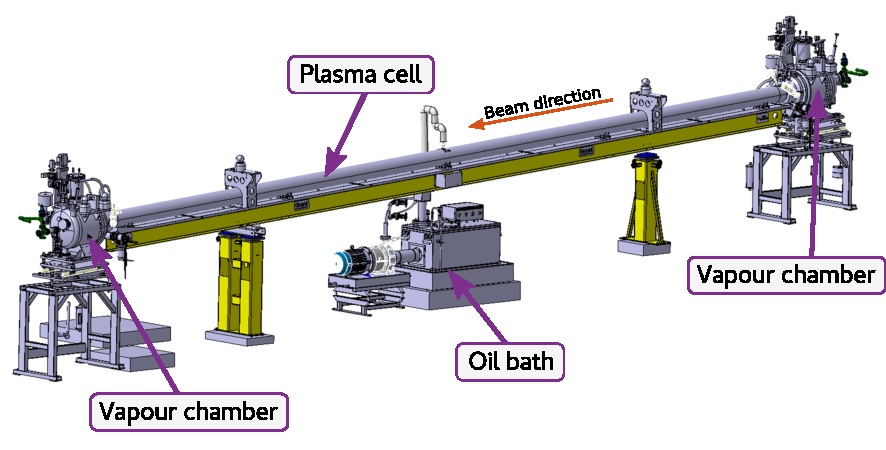
\includegraphics[width=0.99\linewidth,trim={0mm 0mm 0mm 0mm},clip]{figures/PlasmaCell}
    \caption{\label{Fig:WFA:PlasmaCell}
        Drawing of the plasma stage and its related components, as presented in the 2016 AWAKE Status Report~\cite{awake_collaboration:2016}.
    }
\end{figure}

For the AWAKE vapour source, rubidium (Rb) was chosen.
Rubidium has a low melting point, $39.3\celsius$; a low first ionisation energy, $4.18\unit{eV}$; and a standard atomic weight of $85.47$.
The plasma wavelength of rubidium ions with a $+1$ charge is roughly $400$ times that of the plasma electrons (see Equation~\ref{EQ:PWFA:L0W0}), preventing significant ion motion for AWAKE application~\cite{vieira:2012a}.
An additional benefit of using an alkaline metal like rubidium is that the second ionisation level is significantly higher, $27.3\unit{eV}$, making it relatively easy to prevent further ionisation and thus a lower charge/mass ratio~\cite{awake_collaboration:2017}.
The rubidium vapour is created by heating the reservoir and the plasma cell to around $150-230\celsius$ to reach the density range required for AWAKE~\cite{caldwell:2015,muggli:2017a}.

The ionisation of the Rb vapour is achieved with a short laser pulse co-propagating with the proton drive beam.
The laser can be timed such that the plasma channel is created inside the beam itself.
The short laser pulse produces a sharp plasma edge that provides a good seed for the self-modulation instability~\cite{vieira:2014a}, as discussed in Section~\ref{Int:DBeam:SMI}.
The section of the proton beam ahead of the laser does not interact strongly with the neutral rubidium vapour, although a low level of impact ionisation does occur.
However, this effect is not significant~\cite{awake_collaboration:2017}.

The ionisation laser used for AWAKE is a $780\unit{nm}$ Ti:Sapphire laser with a pulse length of $120\unit{fs}$ and a maximum compressed energy of $450\unit{mJ}$.
The peak intensity is around $1.2\nexp{14}\unit{W/cm}^{2}$, with a spot size radius of $1\unit{mm}$~\cite{awake_collaboration:2017}.
The appearance intensity needed for ionisation of rubidium is around $1.7\nexp{12}\unit{W/cm}^{2}$~\cite{augst:1989}.
Ionisation of a second electron requires some $455$ times higher intensity, so secondary ionisation is not expected~\cite{muggli:2017a}.

% Add something about plasma diagnostics, Fabian & Erdem

% ================================================================================================================================ %
\subsection{Electron Source}
\label{WFA:Design:ESource}

The AWAKE electron source for Run~1 consists of a $2.5$ cell RF-gun and a $1\unit{m}$ long booster structure, both operating at $3\unit{GHz}$, a cathode transfer chamber, beam diagnostics, and a beam transport line connecting it to the proton beam line.
The beam is boosted to up to $20\unit{MeV}$ by a constant gradient acceleration structure.
The RF-gun and the booster are powered by a $30\unit{MW}$ klystron~\cite{awake_collaboration:2017,pepitone:2016}.
Several of the components, including the RF-gun and klystron, were re-purposed from the former PHIN injector in the CLIC test facility~\cite{chevallay:2012}.
An overview of the electron source and the accelerating structure can be seen in Figure~\ref{Fig:WFA:ESource}.

\begin{figure}[hbt]
    \centering
    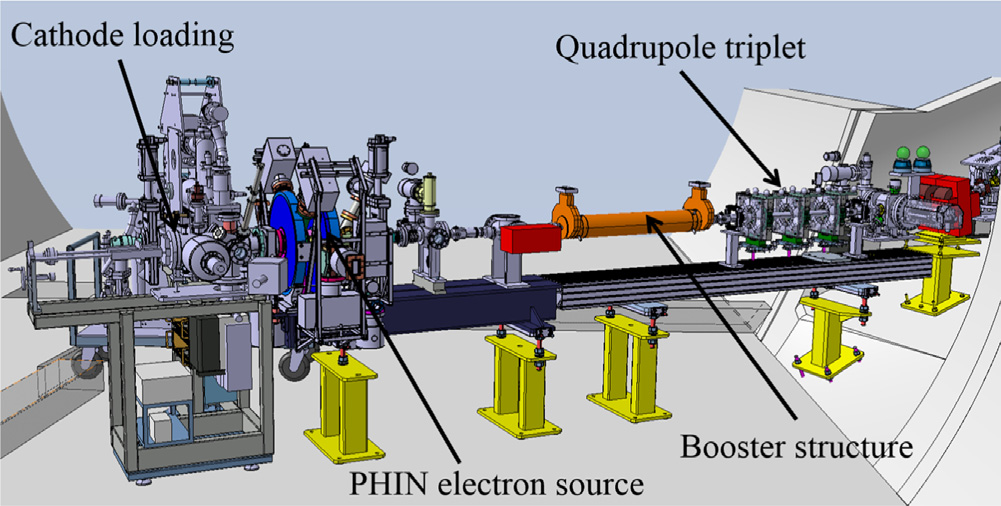
\includegraphics[width=0.70\linewidth,trim={0mm 0mm 0mm 0mm},clip]{figures/ElectronSource}
    \caption{\label{Fig:WFA:ESource}
        Drawing of the electron source and accelerating structure~\cite{pepitone:2016}.
    }
\end{figure}

% ================================================================================================================================ %
\section{Stages of the Experiment}
\label{WFA:AWAKE}

All stages of the AWAKE experiment has been studied in detail in simulations.
Due to the large number of parameters for the plasma and laser, and the drive and witness beams, the range of interest of these have both been determined by previous experiments and AWAKE specific simulations.

\begin{table}[hbt]
    \centering
    \caption{\label{T:AWAKERuns}
        Nominal AWAKE beam parameters for Run~1~\cite{gschwendtner:2014, gschwendtner:2016} and Run~2~\cite{adli:2016a}.
    }
    \begin{tabular}{p{57mm}p{20mm}p{20mm}p{28mm}}
        \rowcolor{tblhead}
        \texthh{Experiment}                   & \texthh{Protons}  & \multicolumn{2}{l}{\texthh{Electrons}}        \\
        \rowcolor{tblunit}
        \texthh{Parameters}                   & \texthu{Run 1\&2} & \texthu{Run 1}    & \texthu{Run 2}            \\
        \hline
        Momentum                              & $400\unit{GeV}$   & $16\unit{MeV}$    & $\gtrsim 50\unit{MeV}$    \\
        Charge                                & $4.8\unit{nC}$    & $200\unit{pC}$    & $67-200\unit{pC}$         \\
        Particles                             & $3\nexp{11}$      & $1.25\nexp{9}$    & $0.42-1.25\nexp{9}$       \\
        Bunch length ($\sigma_{z}$)           & $12\unit{cm}$     & $1.2\unit{mm}$    & $40-60\unit{\mu m}$       \\
        Bunch size ($\sigma_{x,y}$)           & $200\unit{\mu m}$ & $250\unit{\mu m}$ & \textemdash               \\
        Normalised emittance ($\emitN$)       & $3.5\unit{\mu m}$ & $2\unit{\mu m}$   & $\lesssim 10\unit{\mu m}$ \\
        Relative energy spread ($\Delta p/p$) & $0.035\%$         & $0.5\%$           & $\mathrm{few}\,\%$        \\
        Beta function ($\beta^{*}_{x,y}$)     & $4.9\unit{m}$     & $0.4\unit{m}$     & \textemdash               \\
        Dispersion ($D^{*}_{x,y}$)            & $0$               & $0$               & \textemdash               \\
        \hline
    \end{tabular}
\end{table}

The key, nominal parameters for Run~1, and the planned parameters for Run~2, are listed in Table~\ref{T:AWAKERuns}.

% ================================================================================================================================ %
\subsection{AWAKE Run 1}
\label{WFA:AWAKE:R1}

The primary focus of Run~1 of AWAKE was to study the wakefields generated by the SPS proton beam in the $10\unit{m}$ Rubidium plasma stage.
In the first phase the main focus was on measuring the self-modulation instability and the frequency of this modulation in relation to the plasma density.
The second phase aims to sample the generated wakefields with a long electron beam capable of sampling a full plasma wavelength~\cite{adli:2016a}.

A large part of the work involved in Run~1 is related to the operation and diagnostics of all the essential elements involved in the experiment, from the vapour cell and the laser system, to the beam transport; and their respective diagnostics systems.
Especially the size and and density uniformity of the plasma channel are essential parameters to control.

% ================================================================================================================================ %
\subsubsection{The Self-Modulation Instability in AWAKE}
\label{WFA:SMI}

Results from Run 1 of the experiment.

%Karl \cite{rieger:2017}

Does the SMI require a seed? See muggli:2017 \cite{muggli:2017a}.

% ================================================================================================================================ %
\subsection{AWAKE Run 2}
\label{WFA:AWAKE:R2}

% As agreed this is the part you have to expand.  I suggest to add/elaborate the following points

% - why do we need to improve on Run 1 e- acceleration? (Run 1: only long electron beam > lambda_p, in order to sample all phases, also transversally large and unmatched. We therefore expect for Run 1: only a fraction of beam accelerated, large energy spectrum, poor emittance. Run 2 needs to demonstrate that we can accelerate beam interesting for applications, this good emittance, low energy spread, high charge.

% - why do we need to demonstrate scalability? Because single stage acceleration is one of the key advantages with proton driven PWFA. We want to avoid staging as much as possible so you need to rephrase the current text. We might need two plasma stages, one for SSM of the proton beam, and the second for the e- acceleration, but we would like to have ideally only a single stage for the acceleration. For this we need a different kind of plasma source, since we cannot create a laser beam powerful enough for a very long stage, and even if enough energy, it could not propagate through very long distances. You might want to find out why, since one of the opponents is an LWFA experts.  

% The above two points should be sufficient, and will cover 1-2 pages.

% You should end by making clear the segway between what you write here your simulation work: you want to find out whether beam loading can help accelerating an electron beam through long distances with emittance preservation ... and the answer was yes :)

The target objective of Run~2 is the successful acceleration of a short electron beam, looking to maximise energy and charge while retaining a low emittance and energy spread.
In addition, investigating solutions for scaling the experiment to lengths suitable for applications, like for instance a low luminosity electron-proton collider.
One potential solution for such scaling is multiple plasma stages, which may be used for Run~2, although the experimental area has limited space for extending beam lines and adding multiple plasma stages \cite{adli:2016a}.

% ================================================================================================================================ %
